\documentclass[1p]{elsarticle_modified}
%\bibliographystyle{elsarticle-num}

%\usepackage[colorlinks]{hyperref}
%\usepackage{abbrmath_seonhwa} %\Abb, \Ascr, \Acal ,\Abf, \Afrak
\usepackage{amsfonts}
\usepackage{amssymb}
\usepackage{amsmath}
\usepackage{amsthm}
\usepackage{scalefnt}
\usepackage{amsbsy}
\usepackage{kotex}
\usepackage{caption}
\usepackage{subfig}
\usepackage{color}
\usepackage{graphicx}
\usepackage{xcolor} %% white, black, red, green, blue, cyan, magenta, yellow
\usepackage{float}
\usepackage{setspace}
\usepackage{hyperref}

\usepackage{tikz}
\usetikzlibrary{arrows}

\usepackage{multirow}
\usepackage{array} % fixed length table
\usepackage{hhline}

%%%%%%%%%%%%%%%%%%%%%
\makeatletter
\renewcommand*\env@matrix[1][\arraystretch]{%
	\edef\arraystretch{#1}%
	\hskip -\arraycolsep
	\let\@ifnextchar\new@ifnextchar
	\array{*\c@MaxMatrixCols c}}
\makeatother %https://tex.stackexchange.com/questions/14071/how-can-i-increase-the-line-spacing-in-a-matrix
%%%%%%%%%%%%%%%

\usepackage[normalem]{ulem}

\newcommand{\msout}[1]{\ifmmode\text{\sout{\ensuremath{#1}}}\else\sout{#1}\fi}
%SOURCE: \msout is \stkout macro in https://tex.stackexchange.com/questions/20609/strikeout-in-math-mode

\newcommand{\cancel}[1]{
	\ifmmode
	{\color{red}\msout{#1}}
	\else
	{\color{red}\sout{#1}}
	\fi
}

\newcommand{\add}[1]{
	{\color{blue}\uwave{#1}}
}

\newcommand{\replace}[2]{
	\ifmmode
	{\color{red}\msout{#1}}{\color{blue}\uwave{#2}}
	\else
	{\color{red}\sout{#1}}{\color{blue}\uwave{#2}}
	\fi
}

\newcommand{\Sol}{\mathcal{S}} %segment
\newcommand{\D}{D} %diagram
\newcommand{\A}{\mathcal{A}} %arc


%%%%%%%%%%%%%%%%%%%%%%%%%%%%%5 test

\def\sl{\operatorname{\textup{SL}}(2,\Cbb)}
\def\psl{\operatorname{\textup{PSL}}(2,\Cbb)}
\def\quan{\mkern 1mu \triangleright \mkern 1mu}

\theoremstyle{definition}
\newtheorem{thm}{Theorem}[section]
\newtheorem{prop}[thm]{Proposition}
\newtheorem{lem}[thm]{Lemma}
\newtheorem{ques}[thm]{Question}
\newtheorem{cor}[thm]{Corollary}
\newtheorem{defn}[thm]{Definition}
\newtheorem{exam}[thm]{Example}
\newtheorem{rmk}[thm]{Remark}
\newtheorem{alg}[thm]{Algorithm}

\newcommand{\I}{\sqrt{-1}}
\begin{document}

%\begin{frontmatter}
%
%\title{Boundary parabolic representations of knots up to 8 crossings}
%
%%% Group authors per affiliation:
%\author{Yunhi Cho} 
%\address{Department of Mathematics, University of Seoul, Seoul, Korea}
%\ead{yhcho@uos.ac.kr}
%
%
%\author{Seonhwa Kim} %\fnref{s_kim}}
%\address{Center for Geometry and Physics, Institute for Basic Science, Pohang, 37673, Korea}
%\ead{ryeona17@ibs.re.kr}
%
%\author{Hyuk Kim}
%\address{Department of Mathematical Sciences, Seoul National University, Seoul 08826, Korea}
%\ead{hyukkim@snu.ac.kr}
%
%\author{Seokbeom Yoon}
%\address{Department of Mathematical Sciences, Seoul National University, Seoul, 08826,  Korea}
%\ead{sbyoon15@snu.ac.kr}
%
%\begin{abstract}
%We find all boundary parabolic representation of knots up to 8 crossings.
%
%\end{abstract}
%\begin{keyword}
%    \MSC[2010] 57M25 
%\end{keyword}
%
%\end{frontmatter}

%\linenumbers
%\tableofcontents
%
\newcommand\colored[1]{\textcolor{white}{\rule[-0.35ex]{0.8em}{1.4ex}}\kern-0.8em\color{red} #1}%
%\newcommand\colored[1]{\textcolor{white}{ #1}\kern-2.17ex	\textcolor{white}{ #1}\kern-1.81ex	\textcolor{white}{ #1}\kern-2.15ex\color{red}#1	}

{\Large $\underline{12a_{0104}~(K12a_{0104})}$}

\setlength{\tabcolsep}{10pt}
\renewcommand{\arraystretch}{1.6}
\vspace{1cm}\begin{tabular}{m{100pt}>{\centering\arraybackslash}m{274pt}}
\multirow{5}{120pt}{
	\centering
	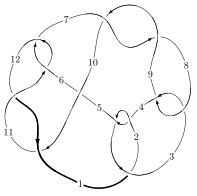
\includegraphics[width=112pt]{../../../GIT/diagram.site/Diagrams/png/905_12a_0104.png}\\
\ \ \ A knot diagram\footnotemark}&
\allowdisplaybreaks
\textbf{Linearized knot diagam} \\
\cline{2-2}
 &
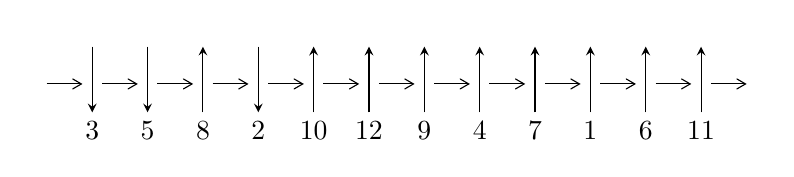
\begin{tikzpicture}[x=20pt, y=17pt]
	% nodes
	\node (C0) at (0, 0) {};
	\node (C1) at (1, 0) {};
	\node (C1U) at (1, +1) {};
	\node (C1D) at (1, -1) {3};

	\node (C2) at (2, 0) {};
	\node (C2U) at (2, +1) {};
	\node (C2D) at (2, -1) {5};

	\node (C3) at (3, 0) {};
	\node (C3U) at (3, +1) {};
	\node (C3D) at (3, -1) {8};

	\node (C4) at (4, 0) {};
	\node (C4U) at (4, +1) {};
	\node (C4D) at (4, -1) {2};

	\node (C5) at (5, 0) {};
	\node (C5U) at (5, +1) {};
	\node (C5D) at (5, -1) {10};

	\node (C6) at (6, 0) {};
	\node (C6U) at (6, +1) {};
	\node (C6D) at (6, -1) {12};

	\node (C7) at (7, 0) {};
	\node (C7U) at (7, +1) {};
	\node (C7D) at (7, -1) {9};

	\node (C8) at (8, 0) {};
	\node (C8U) at (8, +1) {};
	\node (C8D) at (8, -1) {4};

	\node (C9) at (9, 0) {};
	\node (C9U) at (9, +1) {};
	\node (C9D) at (9, -1) {7};

	\node (C10) at (10, 0) {};
	\node (C10U) at (10, +1) {};
	\node (C10D) at (10, -1) {1};

	\node (C11) at (11, 0) {};
	\node (C11U) at (11, +1) {};
	\node (C11D) at (11, -1) {6};

	\node (C12) at (12, 0) {};
	\node (C12U) at (12, +1) {};
	\node (C12D) at (12, -1) {11};
	\node (C13) at (13, 0) {};

	% arrows
	\draw[->,>={angle 60}]
	(C0) edge (C1) (C1) edge (C2) (C2) edge (C3) (C3) edge (C4) (C4) edge (C5) (C5) edge (C6) (C6) edge (C7) (C7) edge (C8) (C8) edge (C9) (C9) edge (C10) (C10) edge (C11) (C11) edge (C12) (C12) edge (C13) ;	\draw[->,>=stealth]
	(C1U) edge (C1D) (C2U) edge (C2D) (C3D) edge (C3U) (C4U) edge (C4D) (C5D) edge (C5U) (C6D) edge (C6U) (C7D) edge (C7U) (C8D) edge (C8U) (C9D) edge (C9U) (C10D) edge (C10U) (C11D) edge (C11U) (C12D) edge (C12U) ;
	\end{tikzpicture} \\
\hhline{~~} \\& 
\textbf{Solving Sequence} \\ \cline{2-2} 
 &
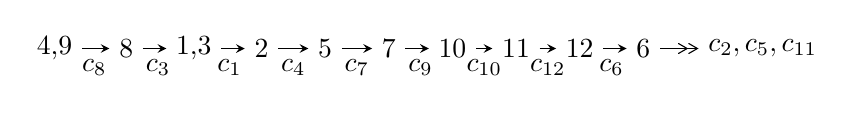
\begin{tikzpicture}[x=23pt, y=7pt]
	% node
	\node (A0) at (-1/8, 0) {4,9};
	\node (A1) at (1, 0) {8};
	\node (A2) at (33/16, 0) {1,3};
	\node (A3) at (25/8, 0) {2};
	\node (A4) at (33/8, 0) {5};
	\node (A5) at (41/8, 0) {7};
	\node (A6) at (49/8, 0) {10};
	\node (A7) at (57/8, 0) {11};
	\node (A8) at (65/8, 0) {12};
	\node (A9) at (73/8, 0) {6};
	\node (C1) at (1/2, -1) {$c_{8}$};
	\node (C2) at (3/2, -1) {$c_{3}$};
	\node (C3) at (21/8, -1) {$c_{1}$};
	\node (C4) at (29/8, -1) {$c_{4}$};
	\node (C5) at (37/8, -1) {$c_{7}$};
	\node (C6) at (45/8, -1) {$c_{9}$};
	\node (C7) at (53/8, -1) {$c_{10}$};
	\node (C8) at (61/8, -1) {$c_{12}$};
	\node (C9) at (69/8, -1) {$c_{6}$};
	\node (A10) at (11, 0) {$c_{2},c_{5},c_{11}$};

	% edge
	\draw[->,>=stealth]	
	(A0) edge (A1) (A1) edge (A2) (A2) edge (A3) (A3) edge (A4) (A4) edge (A5) (A5) edge (A6) (A6) edge (A7) (A7) edge (A8) (A8) edge (A9) ;
	\draw[->>,>={angle 60}]	
	(A9) edge (A10);
\end{tikzpicture} \\ 

\end{tabular} \\

\footnotetext{
The image of knot diagram is generated by the software ``\textbf{Draw programme}" developed by Andrew Bartholomew(\url{http://www.layer8.co.uk/maths/draw/index.htm\#Running-draw}), where we modified some parts for our purpose(\url{https://github.com/CATsTAILs/LinksPainter}).
}\phantom \\ \newline 
\centering \textbf{Ideals for irreducible components\footnotemark of $X_{\text{par}}$} 
 
\begin{align*}
I^u_{1}&=\langle 
1.99116\times10^{67} u^{83}+1.87216\times10^{67} u^{82}+\cdots+3.81065\times10^{67} b+1.15565\times10^{68},\\
\phantom{I^u_{1}}&\phantom{= \langle  }-5.13819\times10^{68} u^{83}-8.03748\times10^{68} u^{82}+\cdots+1.52426\times10^{68} a+6.32981\times10^{69},\;u^{84}+u^{83}+\cdots-20 u+8\rangle \\
\\
I^v_{1}&=\langle 
a,\;v^2+b-2 v+1,\;v^3-2 v^2+v-1\rangle \\
\end{align*}
\raggedright * 2 irreducible components of $\dim_{\mathbb{C}}=0$, with total 87 representations.\\
\footnotetext{All coefficients of polynomials are rational numbers. But the coefficients are sometimes approximated in decimal forms when there is not enough margin.}
\newpage
\renewcommand{\arraystretch}{1}
\centering \section*{I. $I^u_{1}= \langle 1.99\times10^{67} u^{83}+1.87\times10^{67} u^{82}+\cdots+3.81\times10^{67} b+1.16\times10^{68},\;-5.14\times10^{68} u^{83}-8.04\times10^{68} u^{82}+\cdots+1.52\times10^{68} a+6.33\times10^{69},\;u^{84}+u^{83}+\cdots-20 u+8 \rangle$}
\flushleft \textbf{(i) Arc colorings}\\
\begin{tabular}{m{7pt} m{180pt} m{7pt} m{180pt} }
\flushright $a_{4}=$&$\begin{pmatrix}0\\u\end{pmatrix}$ \\
\flushright $a_{9}=$&$\begin{pmatrix}1\\0\end{pmatrix}$ \\
\flushright $a_{8}=$&$\begin{pmatrix}1\\u^2\end{pmatrix}$ \\
\flushright $a_{1}=$&$\begin{pmatrix}3.37094 u^{83}+5.27304 u^{82}+\cdots+31.2513 u-41.5271\\-0.522525 u^{83}-0.491296 u^{82}+\cdots+6.19371 u-3.03269\end{pmatrix}$ \\
\flushright $a_{3}=$&$\begin{pmatrix}- u\\- u^3+u\end{pmatrix}$ \\
\flushright $a_{2}=$&$\begin{pmatrix}2.79271 u^{83}+4.41807 u^{82}+\cdots+23.1737 u-32.5566\\-0.137145 u^{83}+0.0275366 u^{82}+\cdots+13.3625 u-9.78925\end{pmatrix}$ \\
\flushright $a_{5}=$&$\begin{pmatrix}-1.79356 u^{83}-2.91487 u^{82}+\cdots-26.3707 u+29.3430\\-1.57738 u^{83}-2.35817 u^{82}+\cdots-4.88066 u+12.1841\end{pmatrix}$ \\
\flushright $a_{7}=$&$\begin{pmatrix}- u^2+1\\u^2\end{pmatrix}$ \\
\flushright $a_{10}=$&$\begin{pmatrix}u^4- u^2+1\\- u^4\end{pmatrix}$ \\
\flushright $a_{11}=$&$\begin{pmatrix}-1.41045 u^{83}-2.14536 u^{82}+\cdots-1.96825 u+16.7853\\-1.10477 u^{83}-1.62406 u^{82}+\cdots-14.3843 u+13.7098\end{pmatrix}$ \\
\flushright $a_{12}=$&$\begin{pmatrix}3.89508 u^{83}+6.34816 u^{82}+\cdots+35.8388 u-48.8808\\1.62411 u^{83}+2.53617 u^{82}+\cdots+13.9325 u-10.6569\end{pmatrix}$ \\
\flushright $a_{6}=$&$\begin{pmatrix}-2.67160 u^{83}-4.37994 u^{82}+\cdots-30.3466 u+37.6237\\-1.28352 u^{83}-1.99642 u^{82}+\cdots-5.14258 u+10.5210\end{pmatrix}$\\&\end{tabular}
\flushleft \textbf{(ii) Obstruction class $= -1$}\\~\\
\flushleft \textbf{(iii) Cusp Shapes $= 8.77740 u^{83}+13.2937 u^{82}+\cdots+81.5455 u-75.6360$}\\~\\
\newpage\renewcommand{\arraystretch}{1}
\flushleft \textbf{(iv) u-Polynomials at the component}\newline \\
\begin{tabular}{m{50pt}|m{274pt}}
Crossings & \hspace{64pt}u-Polynomials at each crossing \\
\hline $$\begin{aligned}c_{1}\end{aligned}$$&$\begin{aligned}
&u^{84}+48 u^{83}+\cdots+32 u+1
\end{aligned}$\\
\hline $$\begin{aligned}c_{2},c_{4}\end{aligned}$$&$\begin{aligned}
&u^{84}-4 u^{83}+\cdots+8 u-1
\end{aligned}$\\
\hline $$\begin{aligned}c_{3},c_{8}\end{aligned}$$&$\begin{aligned}
&u^{84}+u^{83}+\cdots-20 u+8
\end{aligned}$\\
\hline $$\begin{aligned}c_{5}\end{aligned}$$&$\begin{aligned}
&u^{84}+2 u^{83}+\cdots-34883 u-5113
\end{aligned}$\\
\hline $$\begin{aligned}c_{6},c_{11}\end{aligned}$$&$\begin{aligned}
&u^{84}-2 u^{83}+\cdots+3 u-1
\end{aligned}$\\
\hline $$\begin{aligned}c_{7},c_{9}\end{aligned}$$&$\begin{aligned}
&u^{84}-21 u^{83}+\cdots-1232 u+64
\end{aligned}$\\
\hline $$\begin{aligned}c_{10},c_{12}\end{aligned}$$&$\begin{aligned}
&u^{84}-26 u^{83}+\cdots+5 u+1
\end{aligned}$\\
\hline
\end{tabular}\\~\\
\newpage\renewcommand{\arraystretch}{1}
\flushleft \textbf{(v) Riley Polynomials at the component}\newline \\
\begin{tabular}{m{50pt}|m{274pt}}
Crossings & \hspace{64pt}Riley Polynomials at each crossing \\
\hline $$\begin{aligned}c_{1}\end{aligned}$$&$\begin{aligned}
&y^{84}-20 y^{83}+\cdots-396 y+1
\end{aligned}$\\
\hline $$\begin{aligned}c_{2},c_{4}\end{aligned}$$&$\begin{aligned}
&y^{84}-48 y^{83}+\cdots-32 y+1
\end{aligned}$\\
\hline $$\begin{aligned}c_{3},c_{8}\end{aligned}$$&$\begin{aligned}
&y^{84}-21 y^{83}+\cdots-1232 y+64
\end{aligned}$\\
\hline $$\begin{aligned}c_{5}\end{aligned}$$&$\begin{aligned}
&y^{84}+30 y^{83}+\cdots-376788467 y+26142769
\end{aligned}$\\
\hline $$\begin{aligned}c_{6},c_{11}\end{aligned}$$&$\begin{aligned}
&y^{84}-26 y^{83}+\cdots+5 y+1
\end{aligned}$\\
\hline $$\begin{aligned}c_{7},c_{9}\end{aligned}$$&$\begin{aligned}
&y^{84}+79 y^{83}+\cdots-101632 y+4096
\end{aligned}$\\
\hline $$\begin{aligned}c_{10},c_{12}\end{aligned}$$&$\begin{aligned}
&y^{84}+66 y^{83}+\cdots+53 y+1
\end{aligned}$\\
\hline
\end{tabular}\\~\\
\newpage\flushleft \textbf{(vi) Complex Volumes and Cusp Shapes}
$$\begin{array}{c|c|c}  
\text{Solutions to }I^u_{1}& \I (\text{vol} + \sqrt{-1}CS) & \text{Cusp shape}\\
 \hline 
\begin{aligned}
u &= \phantom{-}0.944843 + 0.334613 I \\
a &= -0.979009 - 0.114566 I \\
b &= \phantom{-}0.193593 - 0.054360 I\end{aligned}
 & \phantom{-}0.240350 + 0.971453 I & \phantom{-0.000000 } 0 \\ \hline\begin{aligned}
u &= \phantom{-}0.944843 - 0.334613 I \\
a &= -0.979009 + 0.114566 I \\
b &= \phantom{-}0.193593 + 0.054360 I\end{aligned}
 & \phantom{-}0.240350 - 0.971453 I & \phantom{-0.000000 } 0 \\ \hline\begin{aligned}
u &= \phantom{-}1.007490 + 0.174190 I \\
a &= -0.175011 - 0.158006 I \\
b &= \phantom{-}0.257564 - 0.954127 I\end{aligned}
 & \phantom{-}1.82802 + 0.02599 I & \phantom{-0.000000 } 0 \\ \hline\begin{aligned}
u &= \phantom{-}1.007490 - 0.174190 I \\
a &= -0.175011 + 0.158006 I \\
b &= \phantom{-}0.257564 + 0.954127 I\end{aligned}
 & \phantom{-}1.82802 - 0.02599 I & \phantom{-0.000000 } 0 \\ \hline\begin{aligned}
u &= -0.919921 + 0.321774 I \\
a &= -0.112585 + 0.178270 I \\
b &= -0.175048 - 1.006520 I\end{aligned}
 & \phantom{-}0.34357 - 3.75775 I & \phantom{-0.000000 } 0 \\ \hline\begin{aligned}
u &= -0.919921 - 0.321774 I \\
a &= -0.112585 - 0.178270 I \\
b &= -0.175048 + 1.006520 I\end{aligned}
 & \phantom{-}0.34357 + 3.75775 I & \phantom{-0.000000 } 0 \\ \hline\begin{aligned}
u &= -1.015960 + 0.163473 I \\
a &= \phantom{-}0.823134 + 0.144319 I \\
b &= \phantom{-}0.048860 + 0.382909 I\end{aligned}
 & \phantom{-}5.40644 - 0.91414 I & \phantom{-0.000000 } 0 \\ \hline\begin{aligned}
u &= -1.015960 - 0.163473 I \\
a &= \phantom{-}0.823134 - 0.144319 I \\
b &= \phantom{-}0.048860 - 0.382909 I\end{aligned}
 & \phantom{-}5.40644 + 0.91414 I & \phantom{-0.000000 } 0 \\ \hline\begin{aligned}
u &= -1.033450 + 0.006740 I \\
a &= \phantom{-}0.530218 - 0.247157 I \\
b &= -0.069544 - 0.793657 I\end{aligned}
 & \phantom{-}2.19629 - 4.45888 I & \phantom{-0.000000 } 0 \\ \hline\begin{aligned}
u &= -1.033450 - 0.006740 I \\
a &= \phantom{-}0.530218 + 0.247157 I \\
b &= -0.069544 + 0.793657 I\end{aligned}
 & \phantom{-}2.19629 + 4.45888 I & \phantom{-0.000000 } 0\\
 \hline 
 \end{array}$$\newpage$$\begin{array}{c|c|c}  
\text{Solutions to }I^u_{1}& \I (\text{vol} + \sqrt{-1}CS) & \text{Cusp shape}\\
 \hline 
\begin{aligned}
u &= -1.020110 + 0.312867 I \\
a &= \phantom{-}1.044500 + 0.003066 I \\
b &= \phantom{-}0.0427561 - 0.0679166 I\end{aligned}
 & \phantom{-}1.06655 - 6.25067 I & \phantom{-0.000000 } 0 \\ \hline\begin{aligned}
u &= -1.020110 - 0.312867 I \\
a &= \phantom{-}1.044500 - 0.003066 I \\
b &= \phantom{-}0.0427561 + 0.0679166 I\end{aligned}
 & \phantom{-}1.06655 + 6.25067 I & \phantom{-0.000000 } 0 \\ \hline\begin{aligned}
u &= \phantom{-}0.337186 + 0.860218 I \\
a &= \phantom{-}0.348190 + 0.078579 I \\
b &= \phantom{-}0.437219 - 0.299567 I\end{aligned}
 & -3.13667 - 6.26179 I & \phantom{-}2.84623 + 7.67334 I \\ \hline\begin{aligned}
u &= \phantom{-}0.337186 - 0.860218 I \\
a &= \phantom{-}0.348190 - 0.078579 I \\
b &= \phantom{-}0.437219 + 0.299567 I\end{aligned}
 & -3.13667 + 6.26179 I & \phantom{-}2.84623 - 7.67334 I \\ \hline\begin{aligned}
u &= \phantom{-}0.794131 + 0.728423 I \\
a &= -0.974458 - 0.845826 I \\
b &= \phantom{-}1.51142 + 0.01992 I\end{aligned}
 & -0.337519 - 0.141011 I & \phantom{-0.000000 } 0 \\ \hline\begin{aligned}
u &= \phantom{-}0.794131 - 0.728423 I \\
a &= -0.974458 + 0.845826 I \\
b &= \phantom{-}1.51142 - 0.01992 I\end{aligned}
 & -0.337519 + 0.141011 I & \phantom{-0.000000 } 0 \\ \hline\begin{aligned}
u &= -0.388919 + 0.818219 I \\
a &= -0.528494 + 0.151733 I \\
b &= -0.219537 - 0.303501 I\end{aligned}
 & -3.73082 + 0.85271 I & \phantom{-}1.01297 - 1.85902 I \\ \hline\begin{aligned}
u &= -0.388919 - 0.818219 I \\
a &= -0.528494 - 0.151733 I \\
b &= -0.219537 + 0.303501 I\end{aligned}
 & -3.73082 - 0.85271 I & \phantom{-}1.01297 + 1.85902 I \\ \hline\begin{aligned}
u &= \phantom{-}1.046740 + 0.346528 I \\
a &= \phantom{-}0.304682 - 0.142438 I \\
b &= \phantom{-}0.289616 - 0.826402 I\end{aligned}
 & \phantom{-}4.27583 + 5.51191 I & \phantom{-0.000000 } 0 \\ \hline\begin{aligned}
u &= \phantom{-}1.046740 - 0.346528 I \\
a &= \phantom{-}0.304682 + 0.142438 I \\
b &= \phantom{-}0.289616 + 0.826402 I\end{aligned}
 & \phantom{-}4.27583 - 5.51191 I & \phantom{-0.000000 } 0\\
 \hline 
 \end{array}$$\newpage$$\begin{array}{c|c|c}  
\text{Solutions to }I^u_{1}& \I (\text{vol} + \sqrt{-1}CS) & \text{Cusp shape}\\
 \hline 
\begin{aligned}
u &= -1.019520 + 0.464975 I \\
a &= -0.631007 + 0.059771 I \\
b &= -0.040704 - 0.556867 I\end{aligned}
 & -1.53401 - 5.48411 I & \phantom{-0.000000 } 0 \\ \hline\begin{aligned}
u &= -1.019520 - 0.464975 I \\
a &= -0.631007 - 0.059771 I \\
b &= -0.040704 + 0.556867 I\end{aligned}
 & -1.53401 + 5.48411 I & \phantom{-0.000000 } 0 \\ \hline\begin{aligned}
u &= -0.832540 + 0.791010 I \\
a &= -1.38296 + 1.38107 I \\
b &= \phantom{-}1.67649 + 0.32338 I\end{aligned}
 & -3.97085 - 1.54693 I & \phantom{-0.000000 } 0 \\ \hline\begin{aligned}
u &= -0.832540 - 0.791010 I \\
a &= -1.38296 - 1.38107 I \\
b &= \phantom{-}1.67649 - 0.32338 I\end{aligned}
 & -3.97085 + 1.54693 I & \phantom{-0.000000 } 0 \\ \hline\begin{aligned}
u &= \phantom{-}0.849652 + 0.031157 I \\
a &= -0.593491 - 0.039522 I \\
b &= \phantom{-}0.386490 + 0.580423 I\end{aligned}
 & \phantom{-}1.276520 - 0.101763 I & \phantom{-}8.75991 - 0.18259 I \\ \hline\begin{aligned}
u &= \phantom{-}0.849652 - 0.031157 I \\
a &= -0.593491 + 0.039522 I \\
b &= \phantom{-}0.386490 - 0.580423 I\end{aligned}
 & \phantom{-}1.276520 + 0.101763 I & \phantom{-}8.75991 + 0.18259 I \\ \hline\begin{aligned}
u &= \phantom{-}1.064990 + 0.457286 I \\
a &= \phantom{-}0.658207 - 0.090830 I \\
b &= \phantom{-}0.215968 - 0.486348 I\end{aligned}
 & -0.60235 + 10.99640 I & \phantom{-0.000000 } 0 \\ \hline\begin{aligned}
u &= \phantom{-}1.064990 - 0.457286 I \\
a &= \phantom{-}0.658207 + 0.090830 I \\
b &= \phantom{-}0.215968 + 0.486348 I\end{aligned}
 & -0.60235 - 10.99640 I & \phantom{-0.000000 } 0 \\ \hline\begin{aligned}
u &= \phantom{-}0.790207 + 0.858708 I \\
a &= -0.96570 - 1.11724 I \\
b &= \phantom{-}2.16628 + 0.31658 I\end{aligned}
 & -6.55489 - 4.86996 I & \phantom{-0.000000 } 0 \\ \hline\begin{aligned}
u &= \phantom{-}0.790207 - 0.858708 I \\
a &= -0.96570 + 1.11724 I \\
b &= \phantom{-}2.16628 - 0.31658 I\end{aligned}
 & -6.55489 + 4.86996 I & \phantom{-0.000000 } 0\\
 \hline 
 \end{array}$$\newpage$$\begin{array}{c|c|c}  
\text{Solutions to }I^u_{1}& \I (\text{vol} + \sqrt{-1}CS) & \text{Cusp shape}\\
 \hline 
\begin{aligned}
u &= -0.885911 + 0.768881 I \\
a &= \phantom{-}1.17335 - 0.91320 I \\
b &= -1.81844 - 0.42053 I\end{aligned}
 & -3.28211 - 2.90476 I & \phantom{-0.000000 } 0 \\ \hline\begin{aligned}
u &= -0.885911 - 0.768881 I \\
a &= \phantom{-}1.17335 + 0.91320 I \\
b &= -1.81844 + 0.42053 I\end{aligned}
 & -3.28211 + 2.90476 I & \phantom{-0.000000 } 0 \\ \hline\begin{aligned}
u &= -0.772200 + 0.886697 I \\
a &= -0.96527 + 1.39186 I \\
b &= \phantom{-}1.68660 - 0.53395 I\end{aligned}
 & -3.85417 + 4.39341 I & \phantom{-0.000000 } 0 \\ \hline\begin{aligned}
u &= -0.772200 - 0.886697 I \\
a &= -0.96527 - 1.39186 I \\
b &= \phantom{-}1.68660 + 0.53395 I\end{aligned}
 & -3.85417 - 4.39341 I & \phantom{-0.000000 } 0 \\ \hline\begin{aligned}
u &= -0.815259 + 0.851759 I \\
a &= \phantom{-}1.02235 - 1.10450 I \\
b &= -2.19830 + 0.15039 I\end{aligned}
 & -7.26044 - 1.06497 I & \phantom{-0.000000 } 0 \\ \hline\begin{aligned}
u &= -0.815259 - 0.851759 I \\
a &= \phantom{-}1.02235 + 1.10450 I \\
b &= -2.19830 - 0.15039 I\end{aligned}
 & -7.26044 + 1.06497 I & \phantom{-0.000000 } 0 \\ \hline\begin{aligned}
u &= \phantom{-}0.826391 + 0.857345 I \\
a &= \phantom{-}1.16777 + 1.50281 I \\
b &= -1.95683 - 0.11611 I\end{aligned}
 & -7.12683 - 1.45321 I & \phantom{-0.000000 } 0 \\ \hline\begin{aligned}
u &= \phantom{-}0.826391 - 0.857345 I \\
a &= \phantom{-}1.16777 - 1.50281 I \\
b &= -1.95683 + 0.11611 I\end{aligned}
 & -7.12683 + 1.45321 I & \phantom{-0.000000 } 0 \\ \hline\begin{aligned}
u &= \phantom{-}0.946159 + 0.729920 I \\
a &= -1.29420 - 0.80499 I \\
b &= \phantom{-}1.58522 - 0.79508 I\end{aligned}
 & \phantom{-}0.12413 + 5.72559 I & \phantom{-0.000000 } 0 \\ \hline\begin{aligned}
u &= \phantom{-}0.946159 - 0.729920 I \\
a &= -1.29420 + 0.80499 I \\
b &= \phantom{-}1.58522 + 0.79508 I\end{aligned}
 & \phantom{-}0.12413 - 5.72559 I & \phantom{-0.000000 } 0\\
 \hline 
 \end{array}$$\newpage$$\begin{array}{c|c|c}  
\text{Solutions to }I^u_{1}& \I (\text{vol} + \sqrt{-1}CS) & \text{Cusp shape}\\
 \hline 
\begin{aligned}
u &= \phantom{-}0.179453 + 0.777420 I \\
a &= \phantom{-}0.311303 - 0.375412 I \\
b &= \phantom{-}0.438005 + 0.193021 I\end{aligned}
 & \phantom{-}1.30918 - 1.58416 I & \phantom{-}9.83805 + 4.37635 I \\ \hline\begin{aligned}
u &= \phantom{-}0.179453 - 0.777420 I \\
a &= \phantom{-}0.311303 + 0.375412 I \\
b &= \phantom{-}0.438005 - 0.193021 I\end{aligned}
 & \phantom{-}1.30918 + 1.58416 I & \phantom{-}9.83805 - 4.37635 I \\ \hline\begin{aligned}
u &= -0.883068 + 0.821610 I \\
a &= -1.54150 + 1.07663 I \\
b &= \phantom{-}2.76029 - 0.11644 I\end{aligned}
 & -10.29460 + 0.43264 I & \phantom{-0.000000 } 0 \\ \hline\begin{aligned}
u &= -0.883068 - 0.821610 I \\
a &= -1.54150 - 1.07663 I \\
b &= \phantom{-}2.76029 + 0.11644 I\end{aligned}
 & -10.29460 - 0.43264 I & \phantom{-0.000000 } 0 \\ \hline\begin{aligned}
u &= -0.710190 + 0.347281 I \\
a &= -2.27716 + 0.25838 I \\
b &= -0.234211 + 0.619343 I\end{aligned}
 & -4.43275 + 1.24589 I & \phantom{-}2.27933 + 1.64914 I \\ \hline\begin{aligned}
u &= -0.710190 - 0.347281 I \\
a &= -2.27716 - 0.25838 I \\
b &= -0.234211 - 0.619343 I\end{aligned}
 & -4.43275 - 1.24589 I & \phantom{-}2.27933 - 1.64914 I \\ \hline\begin{aligned}
u &= -0.937545 + 0.765953 I \\
a &= -1.47040 + 0.78920 I \\
b &= \phantom{-}1.99452 + 0.20653 I\end{aligned}
 & -3.64552 - 4.32145 I & \phantom{-0.000000 } 0 \\ \hline\begin{aligned}
u &= -0.937545 - 0.765953 I \\
a &= -1.47040 - 0.78920 I \\
b &= \phantom{-}1.99452 - 0.20653 I\end{aligned}
 & -3.64552 + 4.32145 I & \phantom{-0.000000 } 0 \\ \hline\begin{aligned}
u &= \phantom{-}0.742303 + 0.267678 I \\
a &= \phantom{-}2.46612 + 0.22285 I \\
b &= \phantom{-}0.453650 + 0.593662 I\end{aligned}
 & -4.02469 + 4.17427 I & \phantom{-}4.30501 - 7.15131 I \\ \hline\begin{aligned}
u &= \phantom{-}0.742303 - 0.267678 I \\
a &= \phantom{-}2.46612 - 0.22285 I \\
b &= \phantom{-}0.453650 - 0.593662 I\end{aligned}
 & -4.02469 - 4.17427 I & \phantom{-}4.30501 + 7.15131 I\\
 \hline 
 \end{array}$$\newpage$$\begin{array}{c|c|c}  
\text{Solutions to }I^u_{1}& \I (\text{vol} + \sqrt{-1}CS) & \text{Cusp shape}\\
 \hline 
\begin{aligned}
u &= -0.910182 + 0.812566 I \\
a &= -1.49098 + 1.66207 I \\
b &= \phantom{-}2.25259 + 0.65273 I\end{aligned}
 & -10.20980 - 6.53851 I & \phantom{-0.000000 } 0 \\ \hline\begin{aligned}
u &= -0.910182 - 0.812566 I \\
a &= -1.49098 - 1.66207 I \\
b &= \phantom{-}2.25259 - 0.65273 I\end{aligned}
 & -10.20980 + 6.53851 I & \phantom{-0.000000 } 0 \\ \hline\begin{aligned}
u &= \phantom{-}0.899767 + 0.828154 I \\
a &= \phantom{-}1.59727 + 1.03673 I \\
b &= -2.77141 + 0.08624 I\end{aligned}
 & -10.97060 + 5.59094 I & \phantom{-0.000000 } 0 \\ \hline\begin{aligned}
u &= \phantom{-}0.899767 - 0.828154 I \\
a &= \phantom{-}1.59727 - 1.03673 I \\
b &= -2.77141 - 0.08624 I\end{aligned}
 & -10.97060 - 5.59094 I & \phantom{-0.000000 } 0 \\ \hline\begin{aligned}
u &= \phantom{-}0.901036 + 0.828606 I \\
a &= \phantom{-}1.42088 + 1.67116 I \\
b &= -2.30109 + 0.49063 I\end{aligned}
 & -10.96750 + 0.58518 I & \phantom{-0.000000 } 0 \\ \hline\begin{aligned}
u &= \phantom{-}0.901036 - 0.828606 I \\
a &= \phantom{-}1.42088 - 1.67116 I \\
b &= -2.30109 - 0.49063 I\end{aligned}
 & -10.96750 - 0.58518 I & \phantom{-0.000000 } 0 \\ \hline\begin{aligned}
u &= \phantom{-}0.822519 + 0.932893 I \\
a &= \phantom{-}0.91684 + 1.64748 I \\
b &= -2.25077 - 0.72210 I\end{aligned}
 & -10.83780 - 3.57887 I & \phantom{-0.000000 } 0 \\ \hline\begin{aligned}
u &= \phantom{-}0.822519 - 0.932893 I \\
a &= \phantom{-}0.91684 - 1.64748 I \\
b &= -2.25077 + 0.72210 I\end{aligned}
 & -10.83780 + 3.57887 I & \phantom{-0.000000 } 0 \\ \hline\begin{aligned}
u &= -0.810693 + 0.944952 I \\
a &= -0.85275 + 1.63282 I \\
b &= \phantom{-}2.19212 - 0.87271 I\end{aligned}
 & -10.04530 + 9.52899 I & \phantom{-0.000000 } 0 \\ \hline\begin{aligned}
u &= -0.810693 - 0.944952 I \\
a &= -0.85275 - 1.63282 I \\
b &= \phantom{-}2.19212 + 0.87271 I\end{aligned}
 & -10.04530 - 9.52899 I & \phantom{-0.000000 } 0\\
 \hline 
 \end{array}$$\newpage$$\begin{array}{c|c|c}  
\text{Solutions to }I^u_{1}& \I (\text{vol} + \sqrt{-1}CS) & \text{Cusp shape}\\
 \hline 
\begin{aligned}
u &= -0.066113 + 0.750316 I \\
a &= \phantom{-}0.110116 - 0.634486 I \\
b &= \phantom{-}0.213608 + 0.726049 I\end{aligned}
 & -2.03059 + 2.74891 I & \phantom{-}4.68139 - 1.77818 I \\ \hline\begin{aligned}
u &= -0.066113 - 0.750316 I \\
a &= \phantom{-}0.110116 + 0.634486 I \\
b &= \phantom{-}0.213608 - 0.726049 I\end{aligned}
 & -2.03059 - 2.74891 I & \phantom{-}4.68139 + 1.77818 I \\ \hline\begin{aligned}
u &= -0.968832 + 0.798968 I \\
a &= \phantom{-}1.37635 - 0.95784 I \\
b &= -2.05317 - 0.97229 I\end{aligned}
 & -6.78392 - 5.08439 I & \phantom{-0.000000 } 0 \\ \hline\begin{aligned}
u &= -0.968832 - 0.798968 I \\
a &= \phantom{-}1.37635 + 0.95784 I \\
b &= -2.05317 + 0.97229 I\end{aligned}
 & -6.78392 + 5.08439 I & \phantom{-0.000000 } 0 \\ \hline\begin{aligned}
u &= \phantom{-}0.965716 + 0.805863 I \\
a &= \phantom{-}1.65828 + 0.77345 I \\
b &= -2.23791 + 0.67188 I\end{aligned}
 & -6.69081 + 7.64283 I & \phantom{-0.000000 } 0 \\ \hline\begin{aligned}
u &= \phantom{-}0.965716 - 0.805863 I \\
a &= \phantom{-}1.65828 - 0.77345 I \\
b &= -2.23791 - 0.67188 I\end{aligned}
 & -6.69081 - 7.64283 I & \phantom{-0.000000 } 0 \\ \hline\begin{aligned}
u &= \phantom{-}0.985942 + 0.791492 I \\
a &= -1.41550 - 0.93253 I \\
b &= \phantom{-}1.99222 - 1.10077 I\end{aligned}
 & -5.94934 + 11.01360 I & \phantom{-0.000000 } 0 \\ \hline\begin{aligned}
u &= \phantom{-}0.985942 - 0.791492 I \\
a &= -1.41550 + 0.93253 I \\
b &= \phantom{-}1.99222 + 1.10077 I\end{aligned}
 & -5.94934 - 11.01360 I & \phantom{-0.000000 } 0 \\ \hline\begin{aligned}
u &= -0.647382 + 0.314500 I \\
a &= \phantom{-}0.331197 + 0.827943 I \\
b &= -0.58409 - 1.80025 I\end{aligned}
 & -4.64480 - 3.92489 I & \phantom{-}3.17496 + 9.60631 I \\ \hline\begin{aligned}
u &= -0.647382 - 0.314500 I \\
a &= \phantom{-}0.331197 - 0.827943 I \\
b &= -0.58409 + 1.80025 I\end{aligned}
 & -4.64480 + 3.92489 I & \phantom{-}3.17496 - 9.60631 I\\
 \hline 
 \end{array}$$\newpage$$\begin{array}{c|c|c}  
\text{Solutions to }I^u_{1}& \I (\text{vol} + \sqrt{-1}CS) & \text{Cusp shape}\\
 \hline 
\begin{aligned}
u &= -1.004740 + 0.795428 I \\
a &= -1.69928 + 0.61945 I \\
b &= \phantom{-}1.90772 + 0.99106 I\end{aligned}
 & -3.12969 - 10.62390 I & \phantom{-0.000000 } 0 \\ \hline\begin{aligned}
u &= -1.004740 - 0.795428 I \\
a &= -1.69928 - 0.61945 I \\
b &= \phantom{-}1.90772 - 0.99106 I\end{aligned}
 & -3.12969 + 10.62390 I & \phantom{-0.000000 } 0 \\ \hline\begin{aligned}
u &= \phantom{-}0.164668 + 0.688630 I \\
a &= -0.154369 - 0.645027 I \\
b &= \phantom{-}0.037509 + 0.772539 I\end{aligned}
 & -2.20909 + 2.50520 I & \phantom{-}4.04658 - 4.39330 I \\ \hline\begin{aligned}
u &= \phantom{-}0.164668 - 0.688630 I \\
a &= -0.154369 + 0.645027 I \\
b &= \phantom{-}0.037509 - 0.772539 I\end{aligned}
 & -2.20909 - 2.50520 I & \phantom{-}4.04658 + 4.39330 I \\ \hline\begin{aligned}
u &= \phantom{-}1.008710 + 0.840149 I \\
a &= \phantom{-}1.86319 + 0.69471 I \\
b &= -2.33246 + 1.32376 I\end{aligned}
 & -10.2365 + 10.1066 I & \phantom{-0.000000 } 0 \\ \hline\begin{aligned}
u &= \phantom{-}1.008710 - 0.840149 I \\
a &= \phantom{-}1.86319 - 0.69471 I \\
b &= -2.33246 - 1.32376 I\end{aligned}
 & -10.2365 - 10.1066 I & \phantom{-0.000000 } 0 \\ \hline\begin{aligned}
u &= -1.020970 + 0.838580 I \\
a &= -1.88269 + 0.64828 I \\
b &= \phantom{-}2.23100 + 1.44321 I\end{aligned}
 & -9.3654 - 16.0858 I & \phantom{-0.000000 } 0 \\ \hline\begin{aligned}
u &= -1.020970 - 0.838580 I \\
a &= -1.88269 - 0.64828 I \\
b &= \phantom{-}2.23100 - 1.44321 I\end{aligned}
 & -9.3654 + 16.0858 I & \phantom{-0.000000 } 0 \\ \hline\begin{aligned}
u &= \phantom{-}0.618250 + 0.265447 I \\
a &= -0.514034 + 0.791465 I \\
b &= \phantom{-}0.89045 - 1.74001 I\end{aligned}
 & -4.45560 - 1.93655 I & \phantom{-}4.71213 - 4.39943 I \\ \hline\begin{aligned}
u &= \phantom{-}0.618250 - 0.265447 I \\
a &= -0.514034 - 0.791465 I \\
b &= \phantom{-}0.89045 + 1.74001 I\end{aligned}
 & -4.45560 + 1.93655 I & \phantom{-}4.71213 + 4.39943 I\\
 \hline 
 \end{array}$$\newpage$$\begin{array}{c|c|c}  
\text{Solutions to }I^u_{1}& \I (\text{vol} + \sqrt{-1}CS) & \text{Cusp shape}\\
 \hline 
\begin{aligned}
u &= \phantom{-}0.622760\phantom{ +0.000000I} \\
a &= \phantom{-}2.68748\phantom{ +0.000000I} \\
b &= \phantom{-}0.499429\phantom{ +0.000000I}\end{aligned}
 & \phantom{-}0.0915949\phantom{ +0.000000I} & \phantom{-}15.1660\phantom{ +0.000000I} \\ \hline\begin{aligned}
u &= -0.273077 + 0.514248 I \\
a &= -1.087230 - 0.760616 I \\
b &= -0.102496 + 0.170604 I\end{aligned}
 & -1.66765 + 0.61770 I & -3.60063 - 1.02986 I \\ \hline\begin{aligned}
u &= -0.273077 - 0.514248 I \\
a &= -1.087230 + 0.760616 I \\
b &= -0.102496 - 0.170604 I\end{aligned}
 & -1.66765 - 0.61770 I & -3.60063 + 1.02986 I \\ \hline\begin{aligned}
u &= \phantom{-}0.458074\phantom{ +0.000000I} \\
a &= -0.459214\phantom{ +0.000000I} \\
b &= \phantom{-}0.469056\phantom{ +0.000000I}\end{aligned}
 & \phantom{-}0.847284\phantom{ +0.000000I} & \phantom{-}12.0560\phantom{ +0.000000I}\\
 \hline 
 \end{array}$$\newpage\newpage\renewcommand{\arraystretch}{1}
\centering \section*{II. $I^v_{1}= \langle a,\;v^2+b-2 v+1,\;v^3-2 v^2+v-1 \rangle$}
\flushleft \textbf{(i) Arc colorings}\\
\begin{tabular}{m{7pt} m{180pt} m{7pt} m{180pt} }
\flushright $a_{4}=$&$\begin{pmatrix}v\\0\end{pmatrix}$ \\
\flushright $a_{9}=$&$\begin{pmatrix}1\\0\end{pmatrix}$ \\
\flushright $a_{8}=$&$\begin{pmatrix}1\\0\end{pmatrix}$ \\
\flushright $a_{1}=$&$\begin{pmatrix}0\\- v^2+2 v-1\end{pmatrix}$ \\
\flushright $a_{3}=$&$\begin{pmatrix}v\\0\end{pmatrix}$ \\
\flushright $a_{2}=$&$\begin{pmatrix}v\\- v^2+2 v-1\end{pmatrix}$ \\
\flushright $a_{5}=$&$\begin{pmatrix}0\\v^2-2 v+1\end{pmatrix}$ \\
\flushright $a_{7}=$&$\begin{pmatrix}1\\0\end{pmatrix}$ \\
\flushright $a_{10}=$&$\begin{pmatrix}1\\0\end{pmatrix}$ \\
\flushright $a_{11}=$&$\begin{pmatrix}1\\- v^2+v+1\end{pmatrix}$ \\
\flushright $a_{12}=$&$\begin{pmatrix}v^2-2 v+1\\- v+1\end{pmatrix}$ \\
\flushright $a_{6}=$&$\begin{pmatrix}v^2-2 v+1\\v^2-2 v+1\end{pmatrix}$\\&\end{tabular}
\flushleft \textbf{(ii) Obstruction class $= 1$}\\~\\
\flushleft \textbf{(iii) Cusp Shapes $= -2 v^2+5 v-1$}\\~\\
\newpage\renewcommand{\arraystretch}{1}
\flushleft \textbf{(iv) u-Polynomials at the component}\newline \\
\begin{tabular}{m{50pt}|m{274pt}}
Crossings & \hspace{64pt}u-Polynomials at each crossing \\
\hline $$\begin{aligned}c_{1},c_{2}\end{aligned}$$&$\begin{aligned}
&(u-1)^3
\end{aligned}$\\
\hline $$\begin{aligned}c_{3},c_{7},c_{8}\\c_{9}\end{aligned}$$&$\begin{aligned}
&u^3
\end{aligned}$\\
\hline $$\begin{aligned}c_{4}\end{aligned}$$&$\begin{aligned}
&(u+1)^3
\end{aligned}$\\
\hline $$\begin{aligned}c_{5},c_{10}\end{aligned}$$&$\begin{aligned}
&u^3+u^2+2 u+1
\end{aligned}$\\
\hline $$\begin{aligned}c_{6}\end{aligned}$$&$\begin{aligned}
&u^3- u^2+1
\end{aligned}$\\
\hline $$\begin{aligned}c_{11}\end{aligned}$$&$\begin{aligned}
&u^3+u^2-1
\end{aligned}$\\
\hline $$\begin{aligned}c_{12}\end{aligned}$$&$\begin{aligned}
&u^3- u^2+2 u-1
\end{aligned}$\\
\hline
\end{tabular}\\~\\
\newpage\renewcommand{\arraystretch}{1}
\flushleft \textbf{(v) Riley Polynomials at the component}\newline \\
\begin{tabular}{m{50pt}|m{274pt}}
Crossings & \hspace{64pt}Riley Polynomials at each crossing \\
\hline $$\begin{aligned}c_{1},c_{2},c_{4}\end{aligned}$$&$\begin{aligned}
&(y-1)^3
\end{aligned}$\\
\hline $$\begin{aligned}c_{3},c_{7},c_{8}\\c_{9}\end{aligned}$$&$\begin{aligned}
&y^3
\end{aligned}$\\
\hline $$\begin{aligned}c_{5},c_{10},c_{12}\end{aligned}$$&$\begin{aligned}
&y^3+3 y^2+2 y-1
\end{aligned}$\\
\hline $$\begin{aligned}c_{6},c_{11}\end{aligned}$$&$\begin{aligned}
&y^3- y^2+2 y-1
\end{aligned}$\\
\hline
\end{tabular}\\~\\
\newpage\flushleft \textbf{(vi) Complex Volumes and Cusp Shapes}
$$\begin{array}{c|c|c}  
\text{Solutions to }I^v_{1}& \I (\text{vol} + \sqrt{-1}CS) & \text{Cusp shape}\\
 \hline 
\begin{aligned}
v &= \phantom{-}0.122561 + 0.744862 I \\
a &= \phantom{-0.000000 } 0 \\
b &= -0.215080 + 1.307140 I\end{aligned}
 & -4.66906 - 2.82812 I & \phantom{-}0.69240 + 3.35914 I \\ \hline\begin{aligned}
v &= \phantom{-}0.122561 - 0.744862 I \\
a &= \phantom{-0.000000 } 0 \\
b &= -0.215080 - 1.307140 I\end{aligned}
 & -4.66906 + 2.82812 I & \phantom{-}0.69240 - 3.35914 I \\ \hline\begin{aligned}
v &= \phantom{-}1.75488\phantom{ +0.000000I} \\
a &= \phantom{-0.000000 } 0 \\
b &= -0.569840\phantom{ +0.000000I}\end{aligned}
 & -0.531480\phantom{ +0.000000I} & \phantom{-}1.61520\phantom{ +0.000000I}\\
 \hline 
 \end{array}$$\newpage
\newpage\renewcommand{\arraystretch}{1}
\centering \section*{ III. u-Polynomials}
\begin{tabular}{m{50pt}|m{274pt}}
Crossings & \hspace{64pt}u-Polynomials at each crossing \\
\hline $$\begin{aligned}c_{1}\end{aligned}$$&$\begin{aligned}
&((u-1)^3)(u^{84}+48 u^{83}+\cdots+32 u+1)
\end{aligned}$\\
\hline $$\begin{aligned}c_{2}\end{aligned}$$&$\begin{aligned}
&((u-1)^3)(u^{84}-4 u^{83}+\cdots+8 u-1)
\end{aligned}$\\
\hline $$\begin{aligned}c_{3},c_{8}\end{aligned}$$&$\begin{aligned}
&u^3(u^{84}+u^{83}+\cdots-20 u+8)
\end{aligned}$\\
\hline $$\begin{aligned}c_{4}\end{aligned}$$&$\begin{aligned}
&((u+1)^3)(u^{84}-4 u^{83}+\cdots+8 u-1)
\end{aligned}$\\
\hline $$\begin{aligned}c_{5}\end{aligned}$$&$\begin{aligned}
&(u^3+u^2+2 u+1)(u^{84}+2 u^{83}+\cdots-34883 u-5113)
\end{aligned}$\\
\hline $$\begin{aligned}c_{6}\end{aligned}$$&$\begin{aligned}
&(u^3- u^2+1)(u^{84}-2 u^{83}+\cdots+3 u-1)
\end{aligned}$\\
\hline $$\begin{aligned}c_{7},c_{9}\end{aligned}$$&$\begin{aligned}
&u^3(u^{84}-21 u^{83}+\cdots-1232 u+64)
\end{aligned}$\\
\hline $$\begin{aligned}c_{10}\end{aligned}$$&$\begin{aligned}
&(u^3+u^2+2 u+1)(u^{84}-26 u^{83}+\cdots+5 u+1)
\end{aligned}$\\
\hline $$\begin{aligned}c_{11}\end{aligned}$$&$\begin{aligned}
&(u^3+u^2-1)(u^{84}-2 u^{83}+\cdots+3 u-1)
\end{aligned}$\\
\hline $$\begin{aligned}c_{12}\end{aligned}$$&$\begin{aligned}
&(u^3- u^2+2 u-1)(u^{84}-26 u^{83}+\cdots+5 u+1)
\end{aligned}$\\
\hline
\end{tabular}\newpage\renewcommand{\arraystretch}{1}
\centering \section*{ IV. Riley Polynomials}
\begin{tabular}{m{50pt}|m{274pt}}
Crossings & \hspace{64pt}Riley Polynomials at each crossing \\
\hline $$\begin{aligned}c_{1}\end{aligned}$$&$\begin{aligned}
&((y-1)^3)(y^{84}-20 y^{83}+\cdots-396 y+1)
\end{aligned}$\\
\hline $$\begin{aligned}c_{2},c_{4}\end{aligned}$$&$\begin{aligned}
&((y-1)^3)(y^{84}-48 y^{83}+\cdots-32 y+1)
\end{aligned}$\\
\hline $$\begin{aligned}c_{3},c_{8}\end{aligned}$$&$\begin{aligned}
&y^3(y^{84}-21 y^{83}+\cdots-1232 y+64)
\end{aligned}$\\
\hline $$\begin{aligned}c_{5}\end{aligned}$$&$\begin{aligned}
&(y^3+3 y^2+2 y-1)(y^{84}+30 y^{83}+\cdots-3.76788\times10^{8} y+2.61428\times10^{7})
\end{aligned}$\\
\hline $$\begin{aligned}c_{6},c_{11}\end{aligned}$$&$\begin{aligned}
&(y^3- y^2+2 y-1)(y^{84}-26 y^{83}+\cdots+5 y+1)
\end{aligned}$\\
\hline $$\begin{aligned}c_{7},c_{9}\end{aligned}$$&$\begin{aligned}
&y^3(y^{84}+79 y^{83}+\cdots-101632 y+4096)
\end{aligned}$\\
\hline $$\begin{aligned}c_{10},c_{12}\end{aligned}$$&$\begin{aligned}
&(y^3+3 y^2+2 y-1)(y^{84}+66 y^{83}+\cdots+53 y+1)
\end{aligned}$\\
\hline
\end{tabular}
\vskip 2pc
\end{document}